\documentclass[times, utf8, diplomski, numeric]{fer}
\usepackage{booktabs}
\usepackage{listings}
\usepackage{color}
\usepackage{pdfpages}



\definecolor{lightgray}{rgb}{.9,.9,.9}
\definecolor{darkgray}{rgb}{.4,.4,.4}
\definecolor{purple}{rgb}{0.65, 0.12, 0.82}

\definecolor{mygreen}{rgb}{0,0.6,0}
\definecolor{mygray}{rgb}{0.5,0.5,0.5}
\definecolor{mymauve}{rgb}{0.58,0,0.82}

\lstset{ %
    backgroundcolor=\color{white}, % choose the background color; you must add \usepackage{color} or \usepackage{xcolor}
    basicstyle=\footnotesize, % the size of the fonts that are used for the code
    breakatwhitespace=false, % sets if automatic breaks should only happen at whitespace
    breaklines=true, % sets automatic line breaking
    captionpos=b, % sets the caption-position to bottom
    commentstyle=\color{mygreen}, % comment style
    deletekeywords={...}, % if you want to delete keywords from the given language
    escapeinside={\%*}{*)}, % if you want to add LaTeX within your code
    extendedchars=true, % lets you use non-ASCII characters; for 8-bits encodings only, does not work with UTF-8
    frame=single, % adds a frame around the code
    keepspaces=true, % keeps spaces in text, useful for keeping indentation of code (possibly needs columns=flexible)
    keywordstyle=\color{blue}, % keyword style
    % language=Octave, % the language of the code
    morekeywords={*,...}, % if you want to add more keywords to the set
    numbers=left, % where to put the line-numbers; possible values are (none, left, right)
    numbersep=5pt, % how far the line-numbers are from the code
    numberstyle=\tiny\color{mygray}, % the style that is used for the line-numbers
    rulecolor=\color{black}, % if not set, the frame-color may be changed on line-breaks within not-black text (e.g. comments (green here))
    showspaces=false, % show spaces everywhere adding particular underscores; it overrides 'showstringspaces'
    showstringspaces=false, % underline spaces within strings only
    showtabs=false, % show tabs within strings adding particular underscores
    stepnumber=1, % the step between two line-numbers. If it's 1, each line will be numbered
    stringstyle=\color{mymauve}, % string literal style
    tabsize=2, % sets default tabsize to 2 spaces
    title=\lstname % show the filename of files included with \lstinputlisting; also try caption instead of title
}
%END of listing package%
 
%define JavaScript language
\lstdefinelanguage{JavaScript}{
    keywords={typeof, new, true, false, function, null, var, in, let, const, class, extends, implements, constructor, super, this, async},
    keywordstyle=\color{blue}\bfseries,  % blue % black
    ndkeywords={import, from, as, export, default, return, if, for, switch, while, do, else, case, break, continue, await, try, catch},
    ndkeywordstyle=\color{purple}\bfseries,  % purple % black
    identifierstyle=\color{black},
    sensitive=false,
    comment=[l]{//},
    morecomment=[s]{/*}{*/},
    commentstyle=\color{green}\ttfamily,  % green % mygray
    stringstyle=\color{red}\ttfamily,  % red % darkgray
    morestring=[b]',
    morestring=[b]"
}
 
\lstset{
    language=JavaScript,
    extendedchars=true,
    basicstyle=\footnotesize\ttfamily,
    showstringspaces=false,
    showspaces=false,
    numbers=left,
    numberstyle=\footnotesize,
    numbersep=9pt,
    tabsize=2,
    breaklines=true,
    showtabs=false,
    captionpos=b
}

\renewcommand{\lstlistingname}{Isječak koda}
\renewcommand{\lstlistlistingname}{Popis isječaka koda}

\newcommand{\razmakp}{\vspace{18pt}}
\newcommand{\razmaks}{\vspace{10pt}}
\newcommand{\uvlakas}{\hspace{0.5cm}}



\begin{document}

\thesisnumber{1937}

\title{Sustav za podršku učenju koncepata deklarativne programske paradigme}

\author{Petar Kovačević}

\maketitle

% Ispis stranice s napomenom o umetanju izvornika rada. Uklonite naredbu \izvornik ako želite izbaciti tu stranicu.
\izvornik

% Dodavanje zahvale ili prazne stranice. Ako ne želite dodati zahvalu, naredbu ostavite radi prazne stranice.
\zahvala{}

\tableofcontents



% Uvod
\chapter{Uvod}

TODO



% Tehnologije
\chapter{Tehnologije}


% Jezik
\section{Jezik}

Programski jezici implementacije sustava su JavaScript za poslužiteljsku stranu \engl{sever-side} i TypeScript za aplikacijsku, odnosno klijentsku stranu \engl{client-side}.
Na klijentskoj strani je u velikoj mjeri prisutna JSX, odnosno TSX sintaksa.

% JavaScript (ECMAScript)
\subsection{JavaScript (ECMAScript)}

JavaScript je viši programski jezik opće namjene koji se primarno izvodi u internet preglednicima, odnosno uz HTML i CSS (koji nisu jezici opće namjene) jedini je programski jezik kojeg preglednici nativno (bez dodataka) podržavaju.
Sintaksa jezika je slična ostalim jezicima takozvane C obitelji jezika, ali za razliku od njih riječ je o dinamičko-tipiziranom \engl{dynamicly typed} interpretabilnom jeziku.\citep{wiki_js}\citep{mdn_js}

Jezik podržava više paradigmi, ali je primarno objektno orijentiran i to, za razliku od drugih popularnih jezika te skupine, baziran na prototipovima \engl{prototype-based}, a ne na razredima.
Ključna razlika između ta dva pristupa je u implementaciji nasljeđivanja. U JavaScript-u se nasljeđivanje odvija proširivanjem \emph{prototipova} koji su posebni tipovi objekata pomoću kojih se stvaraju objekti.\citep{wiki_proto_prog}
Budući da je koncept prototipova većini programera stran i da, zbog dinamičnih tipova u JavaScriptu, neoprezno korištenje može dovesti do nepredviđenih grešaka, od verzije ECMAScript 2015\footnote{
    također poznata pod nazivom ECMAScript 6, skraćeno ES6
} dodani su razredi kao sintaksni šećer \engl{syntax sugar} koje programeri mogu koristiti slično drugim objektno orijentiranim jezicima, a transpilatori\footnote{
    kompilatori, odnosno jezični prevoditelji koji prevode novije verzije JavaScript jezika u starije kako bi stariji preglednici mogli izvršavati napisan kod, primjer: Babel (\url{https://babeljs.io})
} ih prevode u prototipove\citep{mdn_class}.

\razmakp

ECMAScript je pojam koji se često koristi kao alternativno ime za jezik JavaScript, posebice kada se želi naglasiti korištenje modernih novijih verzija jezika.
ECMAScript je ustvari specifikacija skriptnog jezika pod kodovima ECMA-262 i ISO/IEC 16262 kojeg održava međunarodna organizacija Ecma International\footnote{\url{https://www.ecma-international.org}}.
Taj standard implementira više programskih jezika, ali je daleko najpoznatiji JavaScript za kojeg je primarno standard i napisan.
U trenutku pisanja ovog rada najnovija verzija standarda je verzija 9, odnosno ECMAScript 2018.\citep{wiki_es}

% Asinkronost i Promise objekt
\subsubsection{Asinkronost i \emph{Promise} objekt}

Ključan detalj za JavaScript i jezike koje se prevode u JavaScript je da se izvode u jednodretvenom okruženju i da je konkurentnost tog okruženja bazirana na modelu petlje događaja \engl{event loop}.
Pojednostavljena verzija tog modela je da za svaki asinkroni događaj (primjerice dohvat podataka s poslužitelja) postoji funkcija povratnog poziva \engl{callback function} i ta funkcija se stavlja u red poruka \engl{message queue}.
Dretva u kojem se izvršava JavaScript kod je ostvarena kao neblokirajuća beskonačna petlja koja, u trenutku kada ne izvršava neki dio koda, provjerava red poruka.
Ako je asinkron događaj elementa izvađenog iz reda gotov, petlja izvršava funkciju povratnog poziva, inače stavlja događaj nazad u red i provjerava idući element reda.\citep{mdn_event_loop}

\razmakp

U praksi se pokazalo da aplikacijska logika često zahtijeva da se neki asinkron događaj poziva nakon drugog asinkronog događaja, odnosno unutar funkcije povratnog poziva prvog događaja bi se pozivao događaj sa svojom funkcijom povratnog poziva.
Ovakav scenarij se često mogao ponoviti i u toj unutarnjoj funkciji povratnog poziva što bi dovelo do teško održivog i teško čitljivog koda kojeg neki programeri zovu „callback hell“ ili „callback pyramid of doom“.

\razmakp % Primjer ugnježđivanja funkcija povratnog poziva
\begin{lstlisting}[language=JavaScript, caption={Primjer ugnježđivanja funkcija povratnog poziva}, label={lst:callback}]
doSomething(function(result) {
  doSomethingElse(result, function(newResult) {
    doAnotherThing(newResult, function(finalResult) {
      console.log('Got the final result: ' + finalResult);
    }, failureCallback);
  }, failureCallback);
}, failureCallback);
\end{lstlisting}
\razmaks

Rješenje za taj problem je došlo u ECMAScript 2015 uvođenjem \emph{Promise} objekta.
\emph{Promise} je poseban tip objekta koji jer reprezentacija nekog asinkronog događaja, odnosno omotava funkciju povratnog poziva tog asinkronog događaja.
Funkcija je omotana u \emph{obećanje} da će se izvršiti i nad tim objektom može se pozivom metode \emph{then} nizati daljnja \emph{obećanja} asinkronih događaja, odnosno definirati što se izvršava nakon uspješnog ili neuspješnog (metoda \emph{catch}) izvršavanja funkcije povratnog poziva.

\razmakp % Primjer korištenja Promise objekta
\begin{lstlisting}[language=JavaScript, caption={Primjer korištenja \emph{Promise} objekta}, label={lst:promise}]
doSomething()
.then(function(result) {
  return doSomethingElse(result);
})
.then(function(newResult) {
  return doAnotherThing(newResult);
})
.then(function(finalResult) {
  console.log('Got the final result: ' + finalResult);
})
.catch(failureCallback);
\end{lstlisting}
\razmaks

Metode \emph{then} i \emph{catch} su nužne jer \emph{Promise} omotava asinkrone operacije i ne može se izravno iz njega iščitati rezultat operacije jer se u trenutku izvršavanja koda ne zna u kojem je stanju \emph{Promise} objekt.

\begin{figure}[!htb] % Životni ciklus Promise objekta
    \centering
    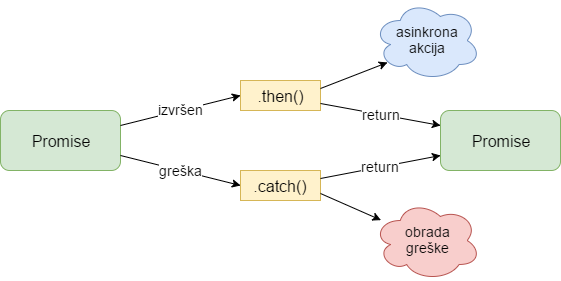
\includegraphics[width=14cm]{images/promise.png}
    \caption{Životni ciklus \emph{Promise} objekta}
    \label{fig:promise_lifecycle}
\end{figure}

\emph{Promise} u svom životnom ciklusu prolazi kroz dva od tri moguća stanja.
Na početku je u pripravnosti \engl{pending} i ovisno o uspješnosti asinkrone operacije odlazi u stanje \emph{ispunjen} \engl{fulfilled} ili \emph{odbijen} \engl{rejected} (vidi sliku \ref{fig:promise_lifecycle}).
U trenutku ulaska u jedno od dva konačna stanja poziva se funkcija ili novi \emph{Promise} definiran kao rezultat funkcije koja je argument \emph{then} ili \emph{catch} metode.
U slučaju da \emph{Promise} uđe u odbijeno stanje, a nema poziva \emph{catch} metode, u aplikaciji će se propagirati greška da odbijeno stanje nije obrađeno \engl{unhandled promise rejection}.\citep{mdn_promise}

\razmakp

Budući da novi koncept \emph{Promise} objekta nije u savršeno pomogao s čitljivošću koda, pogotovo u situacijama kada je nužno obraditi grešku u sredini nekog većeg lanca \emph{Promise} objekata, u specifikaciji ECMAScript 2017 se dodatno uljepšala sintaksa korištenja \emph{Promise} objekata uvođenjem novih ključnih riječi \emph{async} i \emph{await} koji se mogu kombinirati s postojećom \emph{try} i \emph{catch} sintaksom.
Ideja je da se funkcije koje su asinkrone, odnosno vraćaju \emph{Promise} označe ključnom riječi \emph{async}.
Rezultat te funkcije se može odmotati korištenjem ključne riječi \emph{await}.
Time se postiže neblokirajuće čekanje na izvršavanje asinkrone operacije, ekvivalentno tome da se pozvalo \emph{then}.\footnote{
    Transpilator u praksi ne prevodi \emph{await} i kod koji slijedi u \emph{then} već prevodi cijelu \emph{async} funkciju u funkciju generator \engl{generator function} gdje samo \emph{await} zamjeni s \emph{yield“} Ta funkcija generator je potom omotana u drugu funkciju koja koristi taj generator da bi iterirala po koracima lanca asinkronih operacija i pozvala \emph{then} za idući dio lanca. Nakon toga je funkcija generator, budući da je i ona relativno novi dodatak (ECMAScript 2015), prevedena u kod koji je u skladu sa starijim standardom.
}
Za obradu grešaka, umjesto \emph{catch} metode koristi se postojeći \emph{catch} blok.

\razmakp % Primjer korištenja ECMAScript 2017 sintakse
\begin{lstlisting}[language=JavaScript, caption={Primjer korištenja ECMAScript 2017 sintakse}, label={lst:await}]
try {
  const result = await doSomething()
  const newResult = await doSomethingElse(result);
  const finalResult = await doAnotherThing(newResult);
  console.log('Got the final result: ' + finalResult);
} catch (err) {
  failureCallback(err);
}
\end{lstlisting}
\razmaks


% TypeScript
\subsection{TypeScript}

TypeScript je programski jezik razvijen od strane tvrtke Microsoft, koji je nadogradnja \engl{superset} nad jezikom JavaScript.
TypeScript proširuje JavaScript sintaksu \footnote{specifično ECMAScript 2015 i kasnije verzije specifikacije sintakse} s tipovima i sučeljima.
Varijable, konstante, funkcije, razredi i elementi razreda mogu se anotirati prikladnim tipovima čija se ispravnost provjerava pri prevođenju TypeScript koda u JavaScript.
Tipovi mogu biti primitivi (\emph{number}, \emph{boolean}, \emph{string}, \emph{symbol}\footnote{
    \emph{Symbol} je novi JavaScript tip, uveden u ECMAScript 2015 standardu (\url{https://developer.mozilla.org/en-US/docs/Glossary/symbol})
}, \emph{void}), vrijednosti (npr. \emph{null}, \emph{undefined}, \emph{'1'}, \emph{1}, \emph{true}…), objekti (\emph{object}), ugrađeni objekti (npr. \emph{Array}, \emph{Date}, \emph{Function}…), posebni TypeScript tipovi (\emph{any}, \emph{never} i \emph{unknown} \footnote{
    \emph{unknown} je uveden tek u TypeScript verziji 3 kao sigurnija alternativa tipu \emph{any}\citep{ts_3}
}) ili kombinacije spomenutih tipova ostvarenih pomoću sučelja \engl{interface}, unija, presjeka ili kondicionalnih tipova.\citep{gh_ts_spec}\citep{ts_adv}

Korištenje tipova postiže čitljivi i lakše održiv kod,a tipovi omogućavaju se detektiranje nekih čestih JavaScript grešaka pri prevođenju TypeScript koda u JavaScript.\footnote{
    Na JSConf Hawaii konferenciji u veljači 2019 godine je predstavnica tvrtke AirBnB izjavila kako su postmortem analizom svojeg dnevnika grešaka i njihovih ispravaka zaključili da bi migriranje iz JavaScript-a u TypeScript eliminirali 38\% grešaka prije nego što se dese, odnosno pri prevođenju u JavaScript\citep{yt_ts}
}
U nastavku slijedi nekoliko primjera definiranja i korištenja TypeScript tipova.\footnote{
    Napomena: u trenutku pisanja ovog rada najnovija verzija jezika TypeScript je 3.4, no napisani primjeri vrijede i za verziju 2
}

\razmakp % Primjer definiranja i korištenja TypeScript tipova
\begin{lstlisting}[language=JavaScript, caption={Primjer definiranja i korištenja TypeScript tipova}, label={lst:typescript}]
// TODO
\end{lstlisting}
\razmaks

Bitno je napomenuti da korištenje TypeScript jezika ne isključuje mogućnost korištenja čistog JavaScript koda.
Budući da je TypeScript samo nadogradnja na JavaScript, TypeScript datoteke mogu bez ikakvog problema uvoziti \engl{import} JavaScript datoteke i obratno.
Prevoditelj će u takvoj situaciji samo tretirati sve tipove unutar JavaScript datoteke kao tip \emph{any} koji može označavati bilo koji tip, osim ako prevoditelj ima pristup deklaracijskim datotekama \engl{declaration files} za funkcije i varijable koje se izvoze \engl{export} i koriste unutar JavaScript datoteke.
Deklaracijske datoteke su poseban tip TypeScript datoteka \footnote{označavaju se ekstenzijom „.d.ts“} u kojima se nalazi isključivo deklaracije tipova funkcija i objekata koje se koriste u nekoj JavaScript datoteci ili paketu.\citep{ts_declare}
Budući da su većina paketa koje se koriste u razviju TypeScript projekata napisani isključivo u JavaScript kodu, deklaracijske datoteke često se koriste kako bi se opisalo metode tog paketa i održala sigurnost tipova pri prevođenju jezika.
U nastavku slijedi primjer definicije deklaracijske datoteke za neki paket koji nema vlastitu deklaracijsku datoteku.

\razmakp % Primjer deklaracijske datoteke
\begin{lstlisting}[language=JavaScript, caption={Primjer deklaracijske datoteke}, label={lst:declaration_file}]
// TODO
\end{lstlisting}
\razmaks

% JSX i TSX
\subsection{JSX i TSX}

TODO


% Upravljanje paketima
\section{Upravljanje paketima}

% NPM
\subsection{NPM}

TODO

% Semantičko verzioniranje
\subsection{Semantičko verzioniranje}

TODO


% Poslužiteljska strana
\section{Poslužiteljska strana}

TODO

% Node.js
\subsection{Node.js}

TODO

% Express
\subsection{Express}

TODO

% MongoDB
\subsection{MongoDB}

TODO

% Mongoose ODM
\subsection{Mongoose ODM}

TODO


% Aplikacijska (klijentska) strana
\section{Aplikacijska (klijentska) strana}

TODO

% React
\subsection{React}

TODO

% Create React App
\subsection{Create React App}

TODO

% React Router
\subsection{React Router}

TODO

% Redux
\subsection{Redux}

TODO

% STORM React Diagrams
\subsection{STORM React Diagrams}

TODO

% Bootrtarp i React Bootrtarp
\subsection{Bootrtarp i React Bootrtarp}

TODO

% Axios
\subsection{Axios}

TODO



% Specifikacija
\chapter{Specifikacija}


% Opis zadatka
\section{Opis zadatka}

TODO


% Korisnički zahtjevi
\section{Korisnički zahtjevi}

TODO


% Funkcionalni zahtjevi
\section{Funkcionalni zahtjevi}

TODO


% Nefunkcionalni zahtjevi
\section{Nefunkcionalni zahtjevi}

TODO



% Implementacija
\chapter{Implementacija}


% Model podataka
\section{Model podataka}

TODO


% Opis Arhitekture sustava
\section{Opis Arhitekture sustava}

TODO


% Poslužiteljska arhitektura
\section{Poslužiteljska arhitektura}

TODO


% Aplikacijska (klijentska) arhitektura
\section{Aplikacijska (klijentska) arhitektura}

TODO



% Zaključak
\chapter{Zaključak}

TODO




% Literatura
\bibliography{literatura}
\bibliographystyle{fer}

% Sažetak
\begin{sazetak}
Sažetak na hrvatskom jeziku.

\kljucnerijeci{Ključne riječi, odvojene zarezima.}
\end{sazetak}

% TODO: Navedite naslov na engleskom jeziku.
\engtitle{Title}
\begin{abstract}
Abstract.

\keywords{Keywords.}
\end{abstract}

\end{document}
